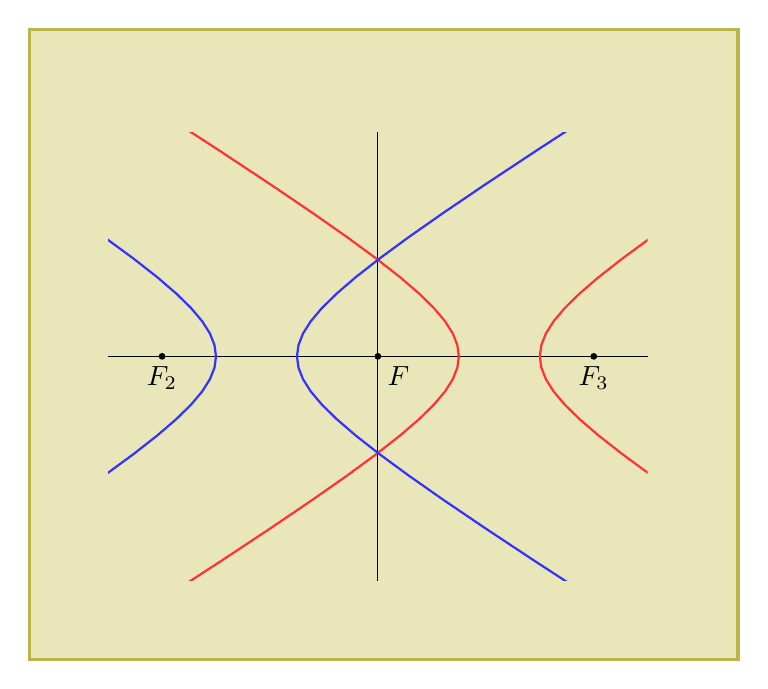
\begin{tikzpicture}
  \draw[draw = olive!60, fill = olive!20, very thick]
    (-1, -1) rectangle (8, 7);

  \begin{axis}[
    xmin = -5,
    xmax = 5,
    ymin = -5,
    ymax = 5,
    axis x line = middle,
    axis y line = middle,
    xlabel = {},
    ylabel = {},
    axis line style = {-},
    ticks = none,
  ]
    \addplot[thick, red!80, domain = -2 : 2]
      ({ 1 + 2 * cosh(x) }, { 1.5 * sinh(x) });
    \addplot[thick, red!80, domain = -2 : 2]
      ({ 3.5 - 2 *  cosh(x) }, { 1.5 * sinh(x) });
    
    \addplot[thick, blue!80, domain = -2 : 2]
      ({ -3.5 + 2 * cosh(x) }, { 1.5 * sinh(x) });
    \addplot[thick, blue!80, domain = -2 : 2]
      ({ -1 - 2 *  cosh(x) }, { 1.5 * sinh(x) });

    \draw (axis cs: 0, 0) node[below right] {\(F\)};
    \draw (axis cs: 4, 0) node[below] {\(F_3\)};
    \draw (axis cs: -4, 0) node[below] {\(F_2\)};

    \draw[fill = black] (axis cs: 0, 0) circle (1pt);
    \draw[fill = black] (axis cs: 4, 0) circle (1pt);
    \draw[fill = black] (axis cs: -4, 0) circle (1pt);
  \end{axis}

\end{tikzpicture}